\section{Условие задания}

Содержание проекта: Команда разработчиков из 16 человек занимается созданием карты города на основе собственного модуля отображения. Проект должен быть завершен в течение 6 месяцев. Бюджет проекта: 50 000 рублей.

\textbf{Дата отчета 5 мая.}

Отметить как выполненные все работы, которые должны были завершиться на эту дату, кроме:

\begin{enumerate}
    \item Задача №6 фактически завершилась 9.04. с 19 марта зарплата 3D-аниматора увеличилась на 20\%.
    \item 5 апреля уволился программист 2, его задачи распределены между программистами 1,3,4 с увеличением их зарплаты на 10\% и увеличением продолжительности стандартного календаря для них на 1 час.
    \item С 12 апреля на 5\% увеличилась стоимость аренды сервера.
    \item Задача №10 выполнена на 80\%.
    \item С 22 марта доступность системного аналитика в проекте снизилась до 80\%.
    \item Фактическая длительность задачи №15 оказалась на 20\% больше.
\end{enumerate}

\section{Задание 1}

По заданию преподавателя была выставлена дата отчета 5 мая.

\begin{figure}[H]
    \centering
    
\includegraphics[width=0.8\textwidth]{img/content/task_1.png}
    \caption{Выставление даты отчета}
    \label{fig:task_1}
\end{figure}

\section{Внесение фактических данных}

По заданию преподавателя были внесены фактические данные выполнения проекта.

\subsection{Повышение зарплаты 3D-аниматора}

С помощью окна обновление задач было выставлено фактическое завершение задачи №6 -- 9 апреля.

С 19 марта была увеличена зарплата 3D-аниматора на 20\%. Данные изменения были внесены в сведениях о ресурсе.

\begin{figure}[H]
    \centering
    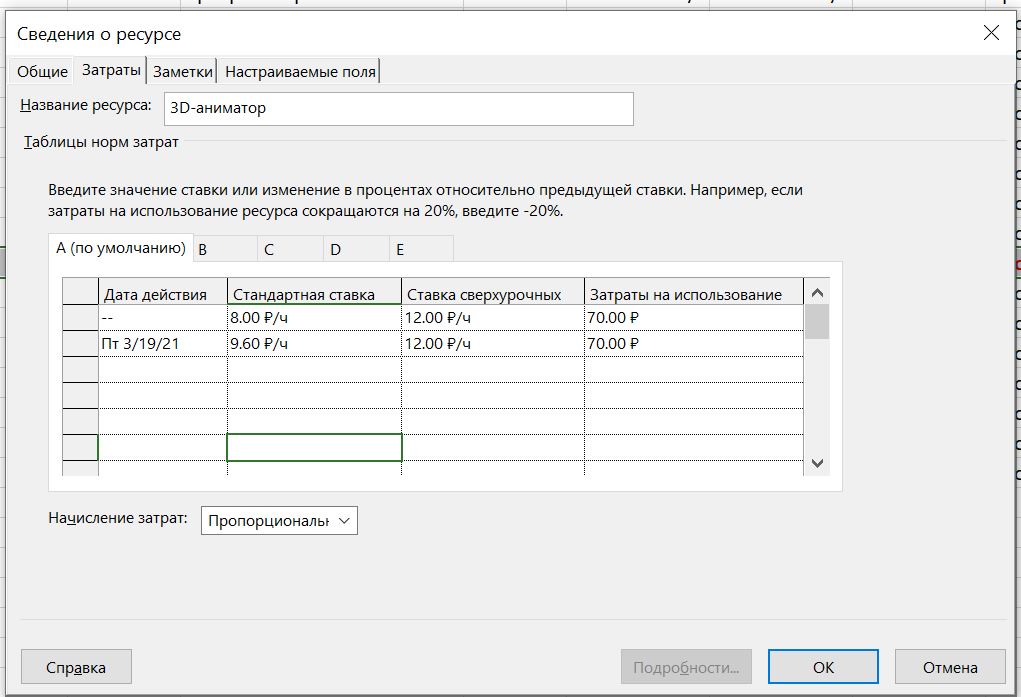
\includegraphics[width=0.8\textwidth]{img/content/1.png}
    \caption{Изменение зарплаты 3D-аниматора}
    \label{fig:1}
\end{figure}

\subsection{Увольнение программиста}

В связи с тем, что программист 2 уволился 5 апреля, потребовалось распределить задачи между остальными программистами с увеличением продолжительности рабочего дня на 1 час и увеличением зарплаты на 10\%.

\begin{figure}[H]
    \centering
    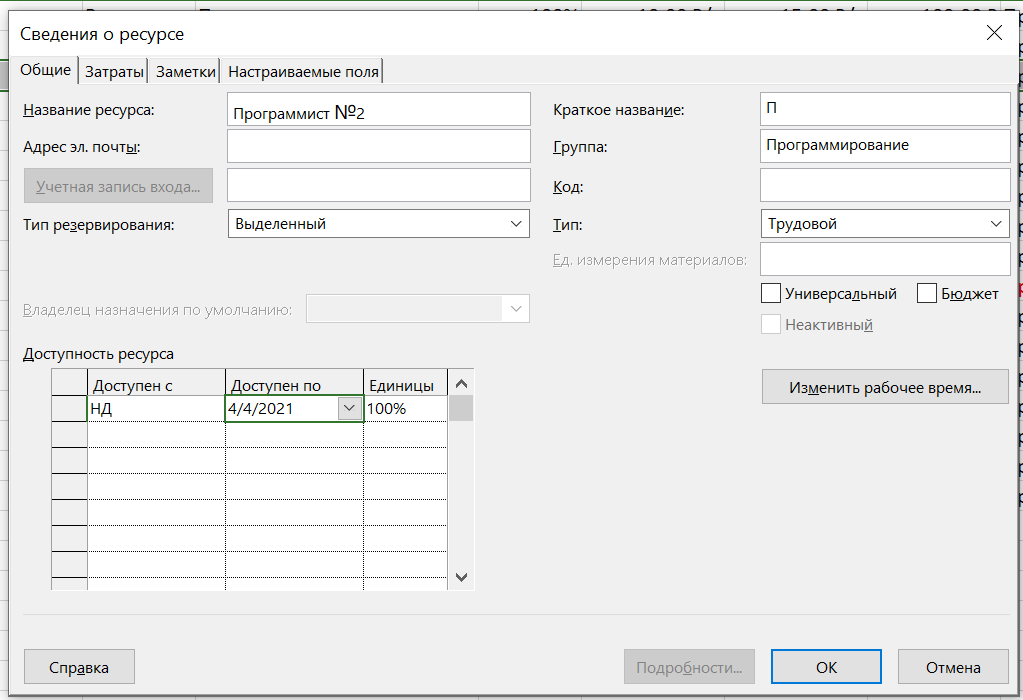
\includegraphics[width=0.8\textwidth]{img/content/2_1.png}
    \caption{Увольнение программиста 2}
    \label{fig:2_1}
\end{figure}

\begin{figure}[H]
    \centering
    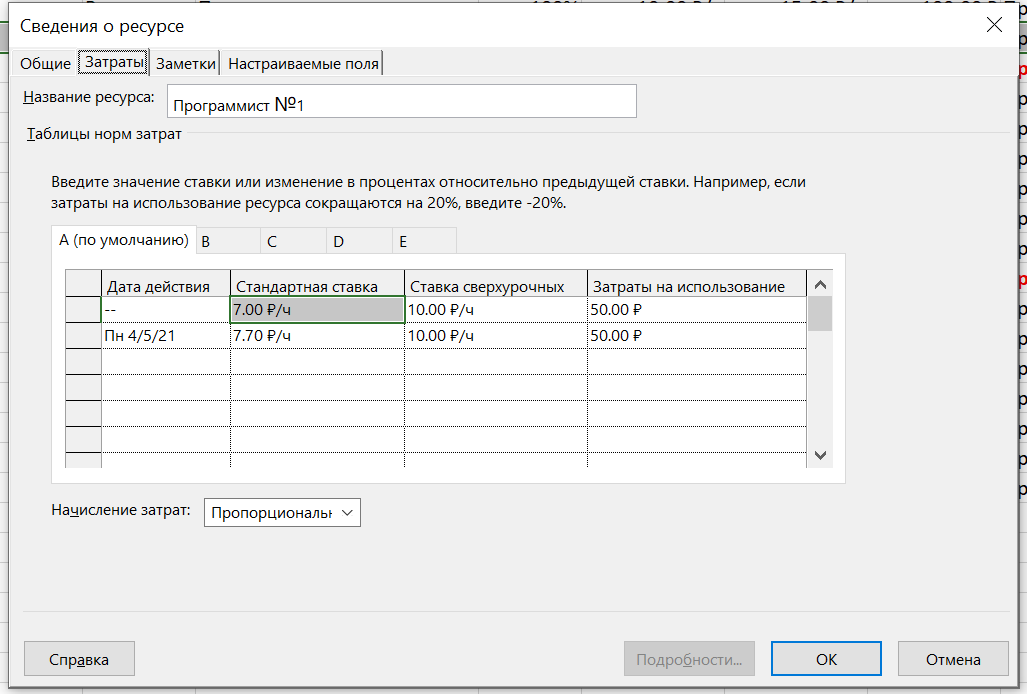
\includegraphics[width=0.8\textwidth]{img/content/2_2.png}
    \caption{Повышение зарплаты остальных программистов на 10\%}
    \label{fig:2_2}
\end{figure}

\begin{figure}[H]
    \centering
    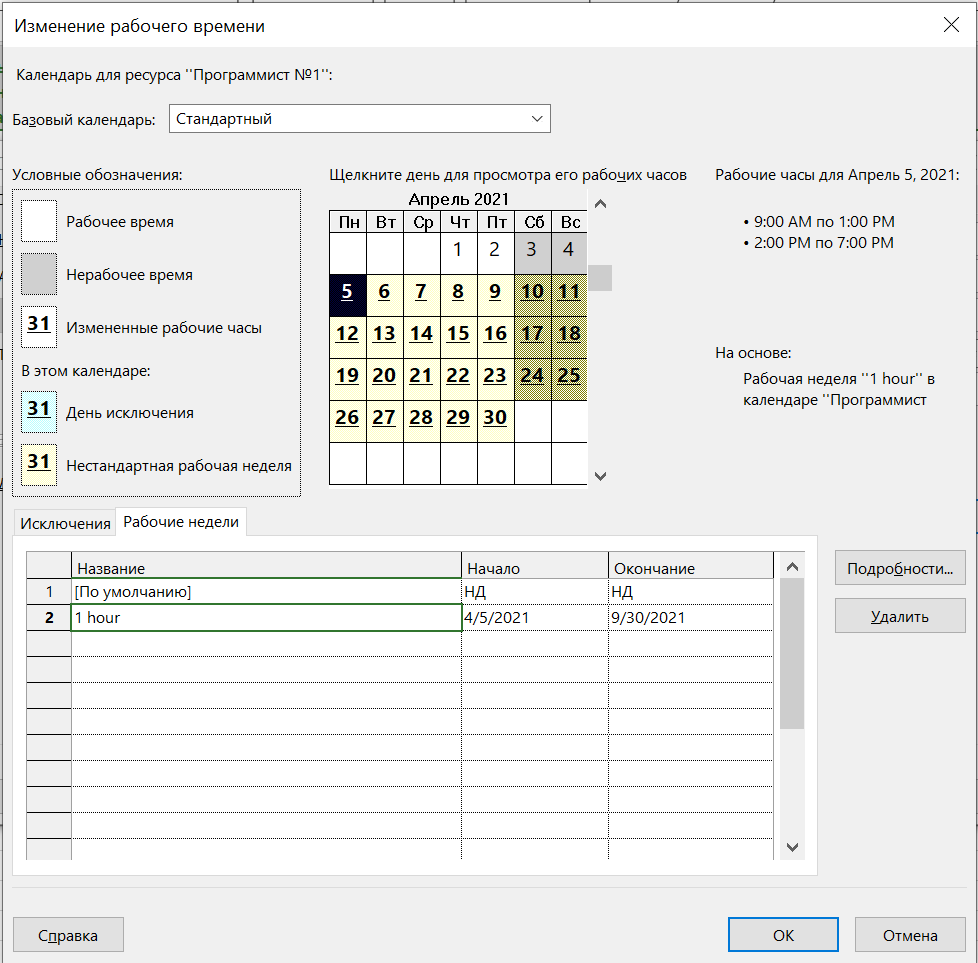
\includegraphics[width=0.8\textwidth]{img/content/2_3.png}
    \caption{Добавление новой рабочей недели для программистов}
    \label{fig:2_3}
\end{figure}

\begin{figure}[H]
    \centering
    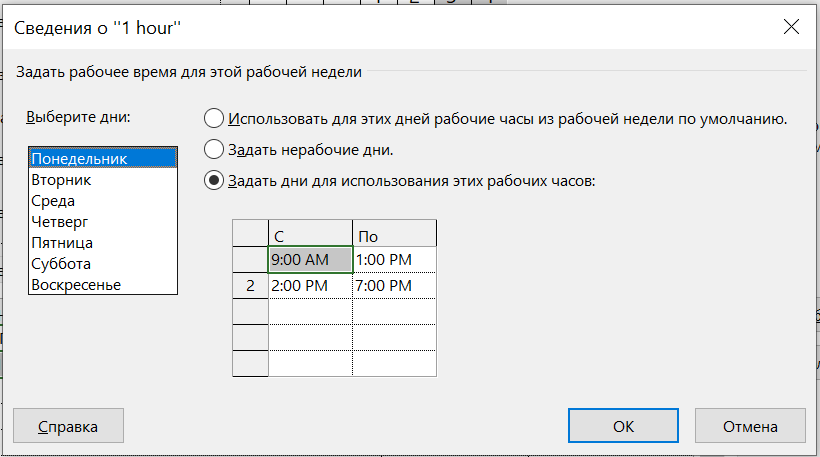
\includegraphics[width=0.8\textwidth]{img/content/2_4.png}
    \caption{Добавление часа в новую рабочую неделю}
    \label{fig:2_4}
\end{figure}

\subsection{Повышение стоимости аренды сервера}

С 12 апреля увеличилась стоимость аренды сервера на 5\%, данная информация была занесена через затраты ресурса.

\begin{figure}[H]
    \centering
    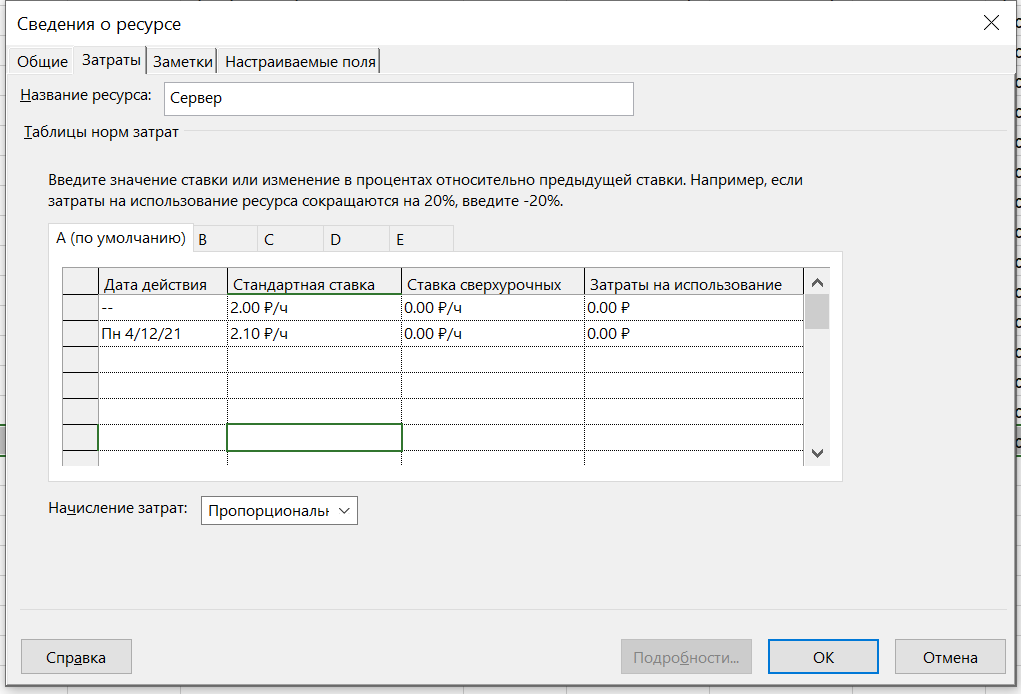
\includegraphics[width=0.8\textwidth]{img/content/3.png}
    \caption{Повышение аренды сервера}
    \label{fig:3}
\end{figure}

\subsection{Выполнение задачи №10}

Задача №10 была выполнена на 80\%. Заносим данные через сведения о задаче.

\begin{figure}[H]
    \centering
    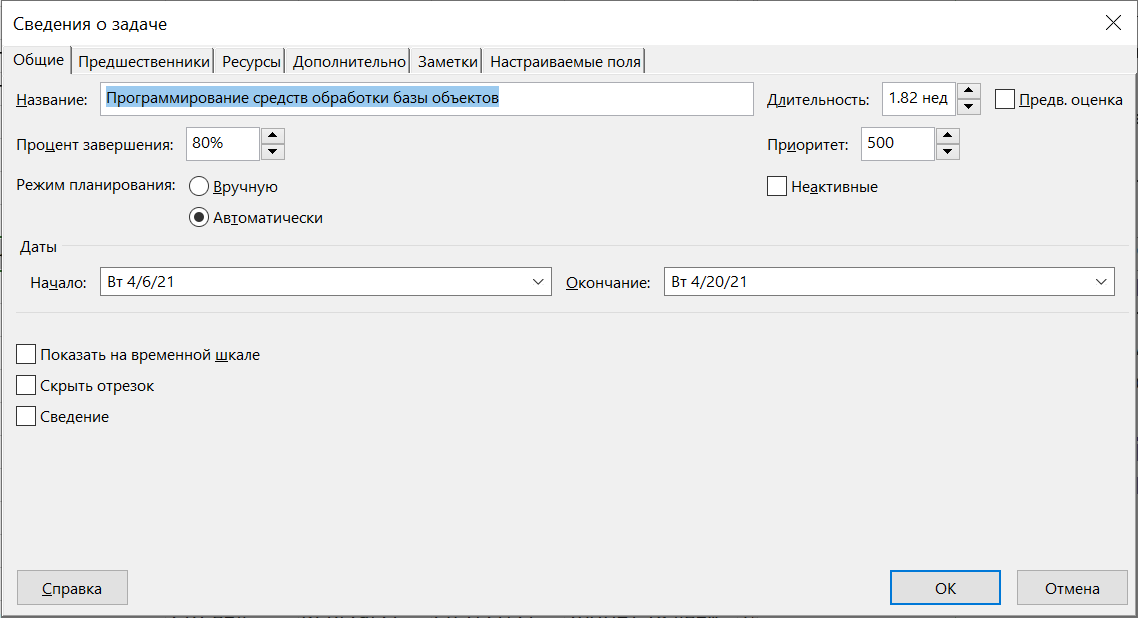
\includegraphics[width=0.8\textwidth]{img/content/4.png}
    \caption{Выполнение задачи на 80\%}
    \label{fig:4}
\end{figure}

\subsection{Доступность системного аналитика}

С 22 марта доступность системного аналитика снизилась до 80\%, что было занесено в сведения о ресурсе.

\begin{figure}[H]
    \centering
    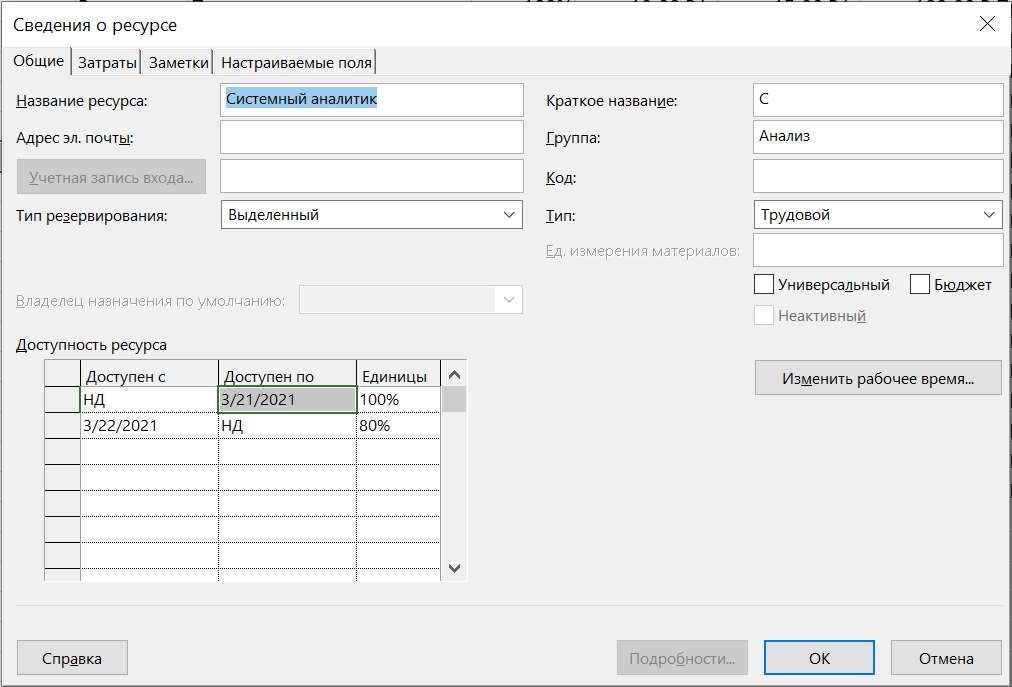
\includegraphics[width=0.8\textwidth]{img/content/5.png}
    \caption{Изменение доступности системного аналитика}
    \label{fig:5}
\end{figure}

\subsection{Длительность задачи №15}

Фактическая длительность задачи №15 оказалась на 20\% больше. Была вычислена новая длительность задачи, которая оказалась равна 1.07 недель, данная информация была занесена в обновление задачи.

\begin{figure}[H]
    \centering
    
\includegraphics[width=0.8\textwidth]{img/content/6.png}
    \caption{Увеличение длительности выполнения задачи №15}
    \label{fig:6}
\end{figure}

\section{Последствия внесения фактических данных}

В результате затраты проекта уменьшились до 48 610 рублей, что укладывается в бюджет 50 000. Завершение проекта сдвинулось до 18 августа, что так же укладывается в рамки плана.

\begin{figure}[H]
    \centering
    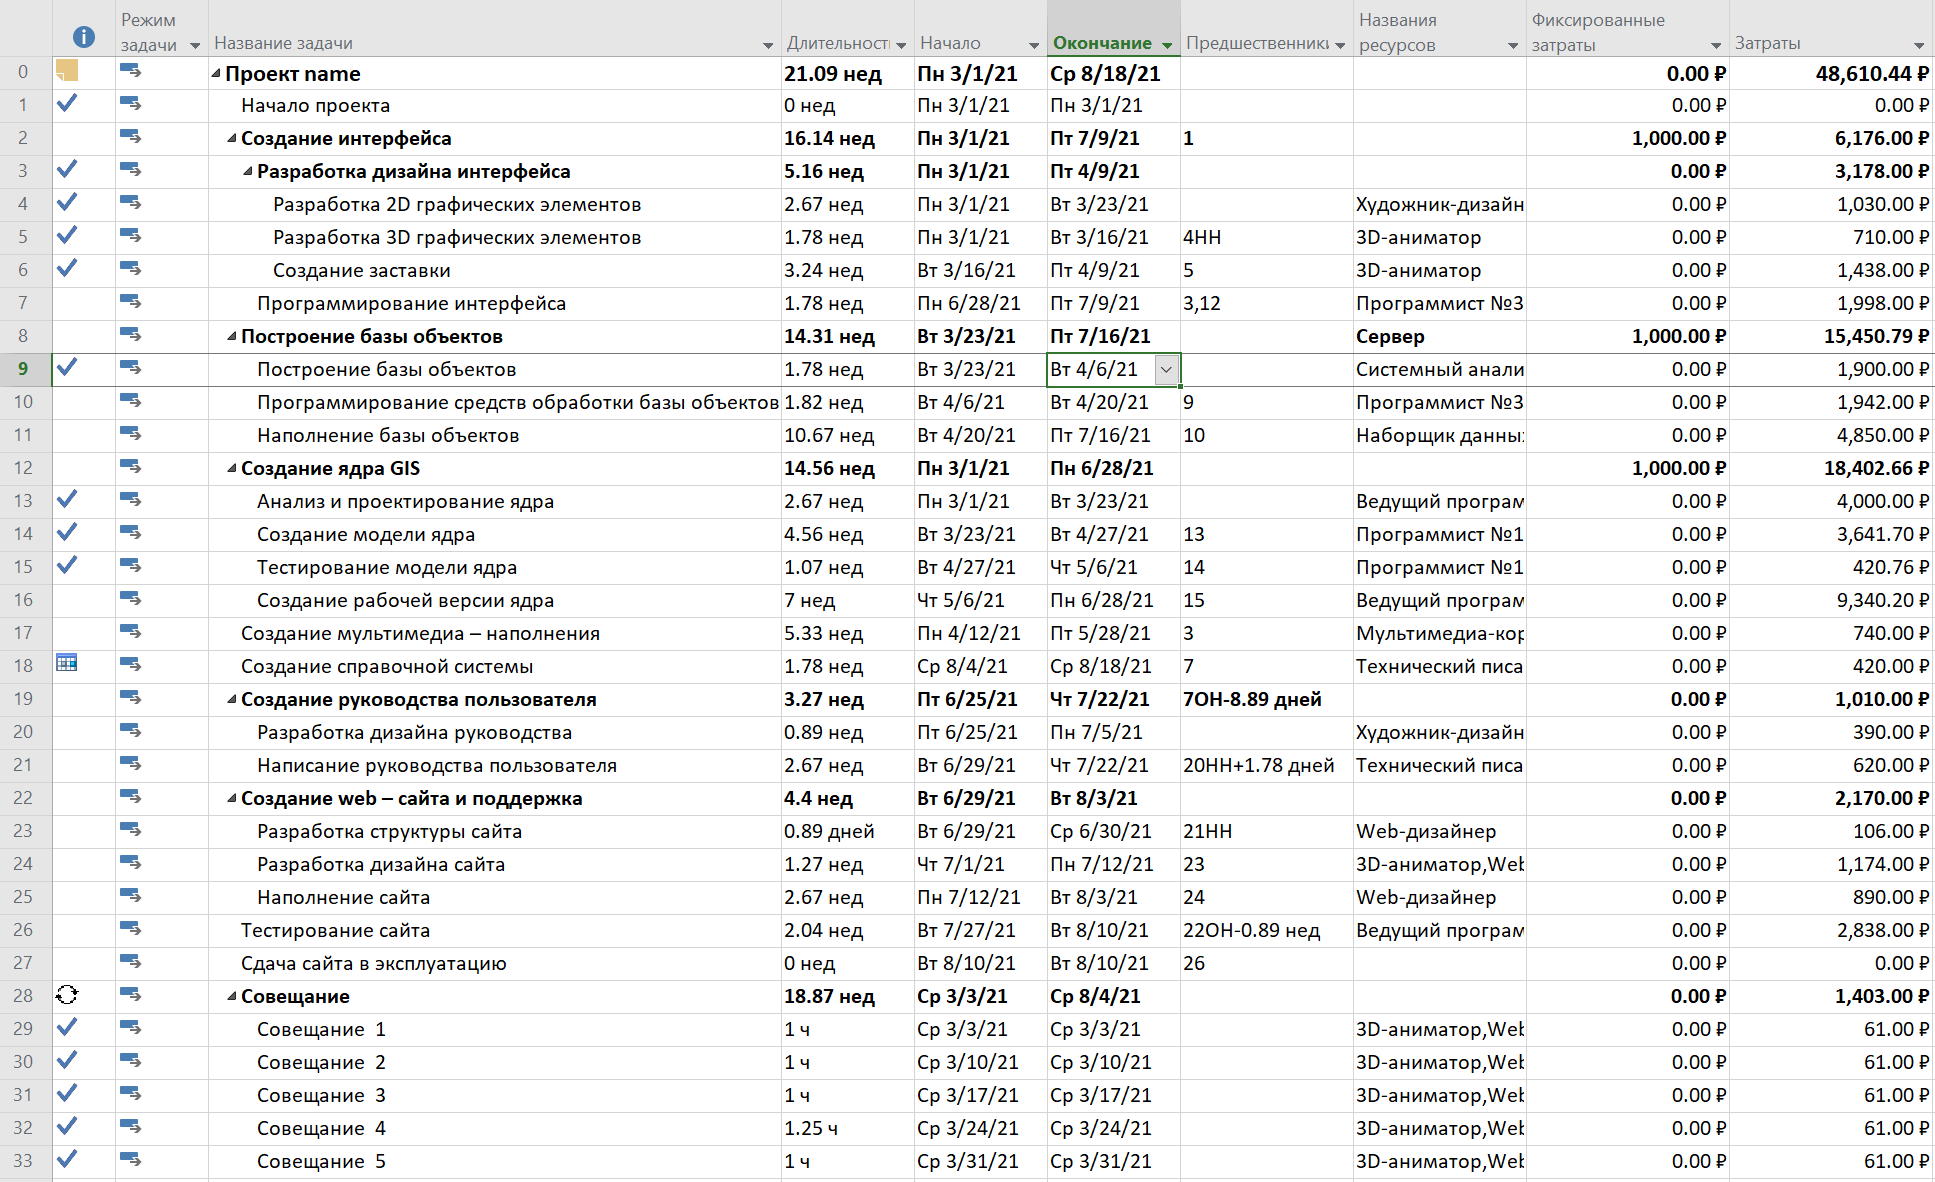
\includegraphics[width=0.8\textwidth]{img/content/final.png}
    \caption{Результат внесения фактических данных}
    \label{fig:final}
\end{figure}

\section{Линия прогресса}

На рисунке \ref{fig:lines} показана линия прогресса выполнения проекта. Видно, что некоторые задачи одут с отставанием.

\begin{figure}[H]
    \centering
    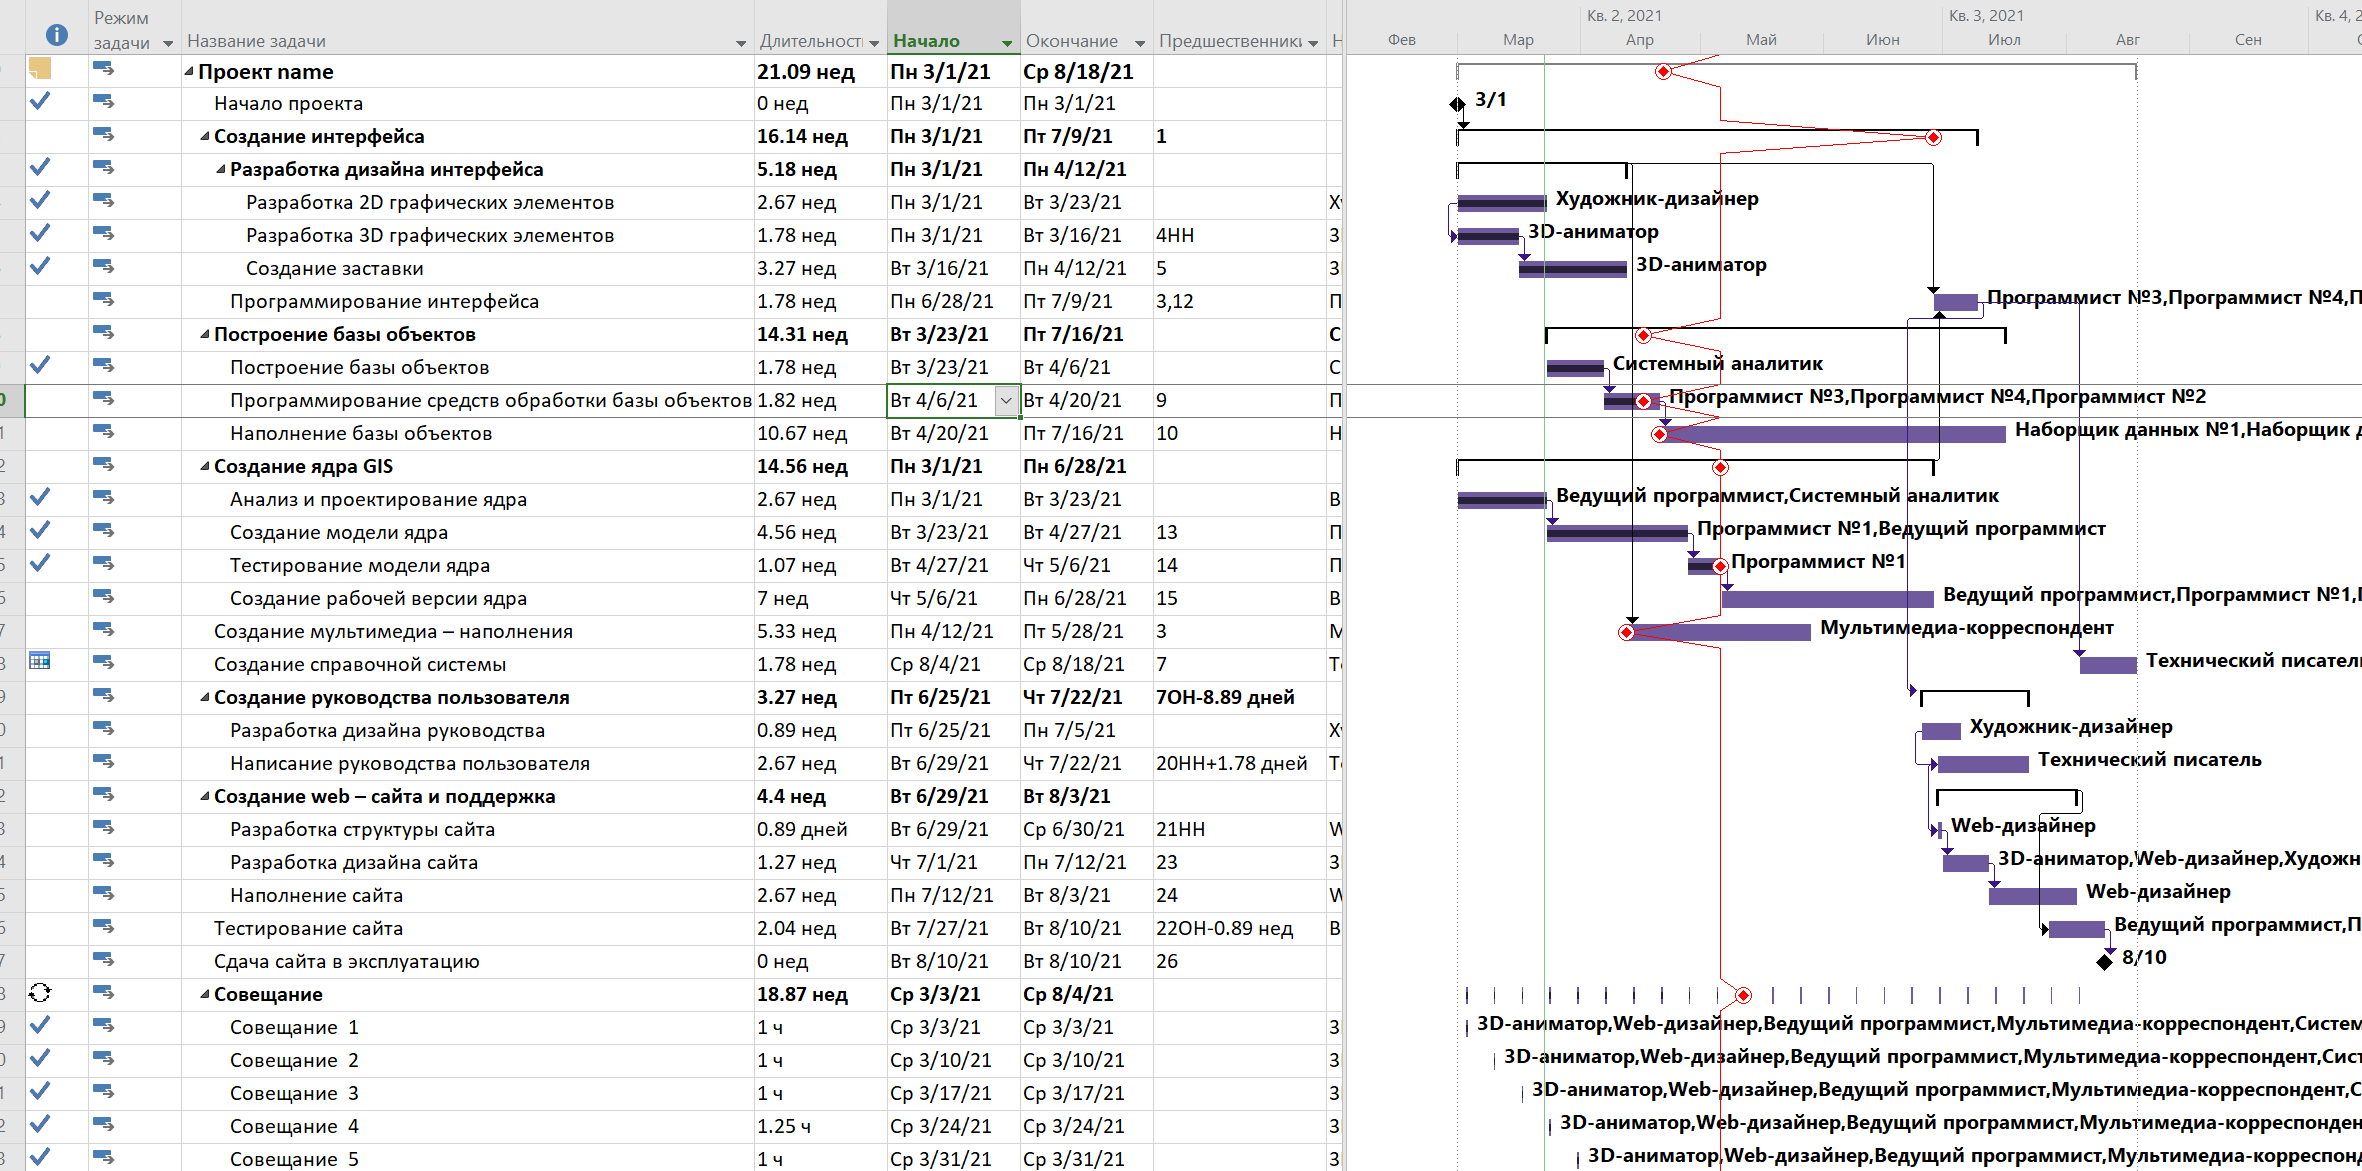
\includegraphics[width=0.8\textwidth]{img/content/lines.png}
    \caption{Линия прогресса проекта}
    \label{fig:lines}
\end{figure}

\section{Выводы}

В результате актуализации состояния проекта оказалось, что реализация от базового плана отличается на 8 дней, то есть срок сдачи составил 18 августа. Бюджет проекта уменьшился до 48 610 рублей.
